\chapter{Evaluation of radiation}\label{evaluation}
In current version of the code following types of radiation are implemented: synchrotron radiation, inverse Compton scattering, gamma-ray emission due to pion decay in free-free proton interaction and also bremsstrahlung.

Для расчета излучения источников используется абстрактный класс RadiationEvaluator и его наследники, предназначенные для конкретных видов излучения. Так же есть класс RadiationSumEvaluator, предназначенный для суммирования нескольких различных видов излучения. Список публичных методов этих двух классов приведен в Таблице \ref{radiationEvaluator}. Общая схема расчета излучения такова: создать источник излучения, используя один из классов описанных в предыдущем разделе или написанный самостоятельно, затем создать вычислитель излучения нужного типа, и вызвать у него метод evaluateFluxFromSource(const double\& photonFinalEnergy, RadiationSource* source), вычисляющий энергетическую плотность потока излучения источника на данной энергии принимаемого фотона в единицах  $\text{см}^{-2} \text{с}^{-1}$. Далее в данном разделе описаны реализации класса RadiationEvaluator для конкретных видов излучения. Схема наследования классов вычислителей излучения представлена на рисунке \ref{radiationEvaluators}. Физическая сторона вопроса, формулы по которым расчитывается излучение подробно описаны в Главе \ref{Formulae}.

\begin{small}
	\topcaption{Публичные методы классa RadiationEvaluator }
	\label{radiationEvaluator}
	\begin{xtabular}{|p{0.5\textwidth}|p{0.5\textwidth}|} 
		\hline
		\textbf{RadiationEvaluator} & абстрактный класс для вычисления излучения \\
		\hline
		virtual evaluateFluxFromSource(const double\& photonFinalEnergy, RadiationSource* source) & чисто виртуальный метод, возвращает энергетическую плотность потока излучаемого данным источником в единицах $\text{см}^{-2} \text{с}^{-1}$ \\
		\hline
		virtual double evaluateFluxFromSourceAtPoint(const double\& photonFinalEnergy, RadiationSource* source, int rhoi, int phi) & чисто виртуальный метод, возвращает энергетическую плотность потока, излучаемого данной областью источника на картинной плоскости\\
		double evaluateTotalFluxInEnergyRange(const double\& Ephmin, const double\& Ephmax, int Nph, RadiationSource* source) & возвращает интегральны поток излучаемый источником в заданном диапазоне энергий (проинтегрированный по Nph точкам) в единицах  $\text{эрг} \text{см}^{-2} \text{с}^{-1}$\\
		\hline
		virtual resetParameters( const double* parameters, const double* normalizationUnits) & чисто виртуальный метод, позволяет изменить внутренние параметры вычислителя излучения. Список параметров, их количество, их влияние на источник определяются  в конкретных реализациях класса, данный метод используется при оптимизации\\
		\hline
		writeFluxFromSourceToFile(const char* fileName, RadiationSource* source, const double\& Ephmin, const double\& Ephmax, const int Nph) & записывает в файл с данным именем излучение источника в единицах $\text{см}^{-2} \text{с}^{-1}$ в диапазоне от минимальной до максимальной энергии, с заданным количеством точек, распределенных логарифмически\\
		\hline
		void writeImageFromSourceToFile(const char* fileName, RadiationSource* source, const double\& Ephmin, const double\& Ephmax, const int Nph) & записывает в файл с данным именем изображение - двумерный массив с интегральным потоком излучаемым разными областями источника в единицах $\text{эрг} \text{см}^{-2} \text{с}^{-1}$ в диапазоне от минимальной до максимальной энергии, проинтегрированым по заданныму количеству точек, распределенных логарифмически\\
		\hline
		void writeImageFromSourceAtEToFile(const double\& photonFinalEnergy, const char* fileName, RadiationSource* source) & записывает в файл с данным именем изображение - двумерный массив с энергетической плотностью потока излучаемого разными областями источника на данных энергиях в единицах $\text{см}^{-2} \text{с}^{-1}$\\
		\hline
		\textbf{RadiationSumEvaluator} & класс предназначенный для суммирования нескольких видов излучения\\
		\hline
		RadiationSumEvaluator(int Ne, const double\& Emin, const double\& Emax, RadiationEvaluator* evaluator1, RadiationEvaluator* evaluator2) & конструктор, создающий экземпляр с указанным диапазоном рассматриваемых энергий излучающих частиц, вычисляющий и складывающий результаты двух указанных вычислителей \\
		\hline
		RadiationSumEvaluator(int Ne, const double\& Emin, const double\& Emax, int Nev, RadiationEvaluator** evaluators) & конструктор, создающий экземпляр с указанным диапазоном рассматриваемых энергий излучающих частиц, вычисляющий и складывающий результаты вычислителей излучения в указанном массиве\\
		\hline
	\end{xtabular}
\end{small}

\begin{figure}[h]
	\centering
	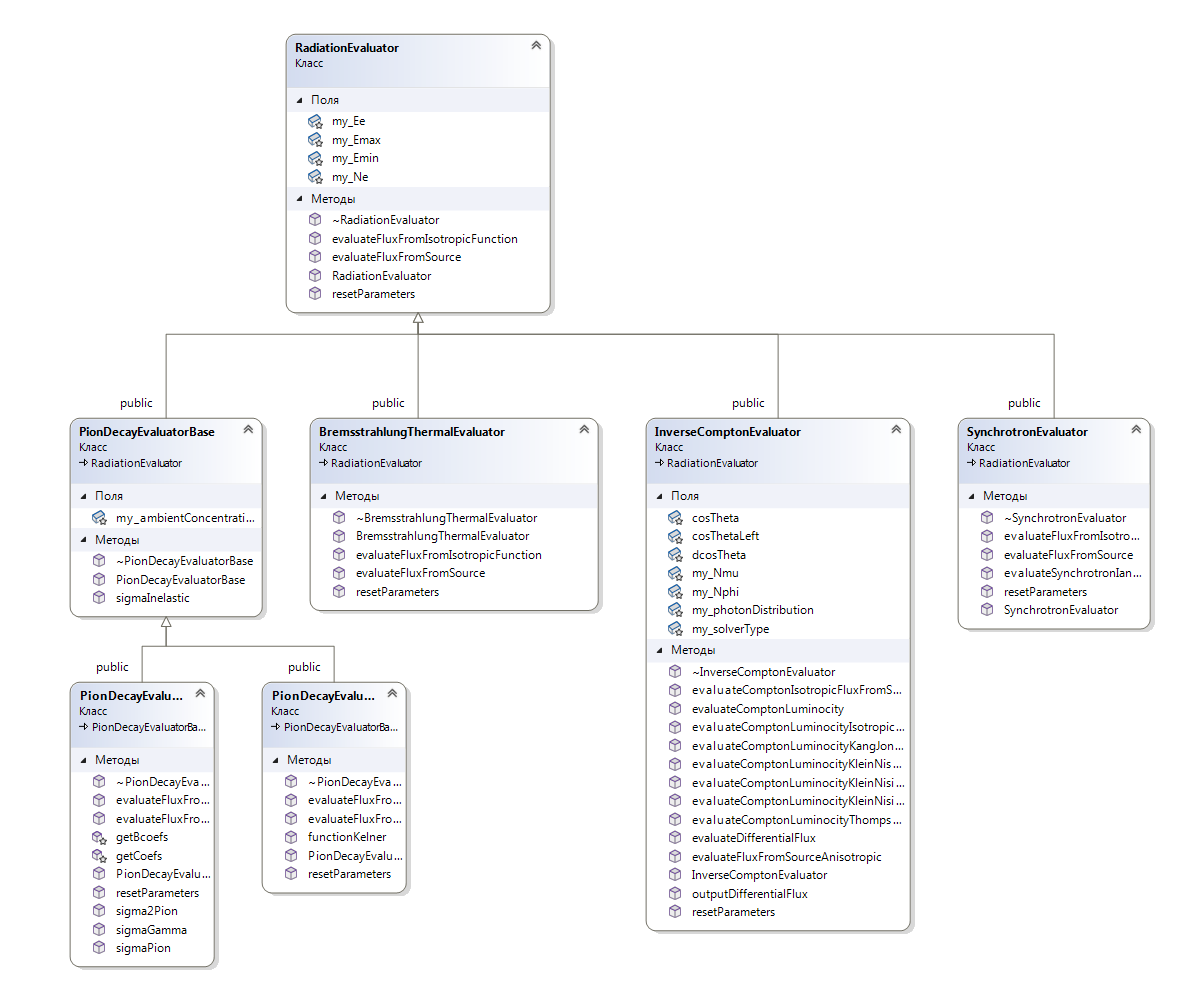
\includegraphics[width=10.5 cm]{./fig/radiationEvaluator.png} 
	\caption{Схема наследования классов вычислителей излучения.}
	\label{radiationEvaluators}
\end{figure}

\section{Синхротронное излучение}
Для расчета синхротронного излучения используется класс SynchrotronEvaluator. В нем используется приближение непрерывного спектра, то есть рассматриваемые частоты фотонов предполагаются намного большими, чем частота вращения излучающих частиц в магнитном поле. Реализован случай только изотропной функции распределения излучающих частиц. Так же возможен учет синхротронного самопоглощения. Используемая геометрия источников, показанная на рисунке \ref{sphericalLayer}, позволяет легко интегрировать излучение по лучу зрения, и учитывать при этом поглощение внутри источника. При создании объекта класса необходимо указать рассматриваемый диапазон энергий частиц и количество точек в нем, параметр отвечающий за учет самопоглощения (значение по умолчанию true), а так же значения магнитного поля, синуса угла наклона к лучу зрения и толщины излучаемой области, которые будут использоваться в случае расчета излучения без указания источника, а только с использованием распределения частиц. Публичные методы класса SynchrotronEvaluator перечислены в Таблице \ref{SynchrotronEvaluator}. Пример вычисления синхотронного излучения приведен в разделе \ref{quickStart}.
\begin{table}
	\begin{center}
	\begin{small}
	\caption{Публичные методы классa SynchrotronEvaluator }
	\label{SynchrotronEvaluator}
	\begin{tabularx}{\textwidth}{|X|X|} 
		\hline
		\textbf{SynchrotronEvaluator} & класс предназначенный для вычисления синхротронного излучения\\
		\hline
		SynchrotronEvaluator( int Ne, double Emin, double Emax, bool selfAbsorption = true, bool doppler = false) & конструктор, создает экземпляр с указанным диапазоном рассматриваемых энергий излучающих частиц,и параметрами учета самопоглощения и допплеровского эффекта\\
		\hline
		evaluateSynchrotronIandA(const double\& photonFinalFrequency, const double\& photonFinalTheta, const double\& photonFinalPhi, const double\& B, const double\& sinhi, const double\& concentration, MassiveParticleIsotropicDistribution* electronDistribution, double\& I, double\& A) & вычисляет значения плотности излучательной способности и коэффициента поглощения для фотона с данной энергией и направлением, в области с данными концентрацией и распределением излучающих частиц в данном магнитном поле\\
		\hline
	\end{tabularx}
\end{small}
\end{center}
\end{table}
\section{Обратное комптоновское рассеяние}
Для расчета излучения, получающегося в результате процесса обратного комптоновского рассеяния, использеуются классы InverseComptonEvaluator и его наследник InverseComptonEvaluatorWithSource. Отличие между ними в том, что в первом функция распределения рассеиваемых фотонов одинакова во всем излучающем объеме, а во втором изменяется обратно пропорционально квадрату расстояния до источника фотонов. Внутри класса  InverseComptonEvaluator реализованы четыре различных метода расчета излучения, для обозначения которых используется перечислимый тип ComptonSolverType, имеющий следующие значения:

\begin{itemize}
	\item ISOTROPIC\_THOMSON - модель рассеяния в томсоновсков режиме. Реализовано только для степенного распределения электронов и теплового фотонов \cite{Ginzburg1975} глава 17, с. 466
	\item ANISOTROPIC\_KLEIN\_NISHINA - модель расчитывающее излучение напрямую из сечения Клейна-Нишины, возможен учет анизотропных функций распределения \cite{KleinNishina, Dubus}
	\item ISOTROPIC\_KLEIN\_NISHINA - модель расчитывающее излучение напрямую из сечения Клейна-Нишины, но для изотропных функций распределения, что позволяет уменьшить количество интегрирований
	\item ISOTROPIC\_JONES - модель, использующая аналитически проинтегрированное по углам сечение Клейна-Нишины \cite{JonesCompton, BykovUvarov2000}
\end{itemize}

При создании объекта класса InverseComptonEvaluator необходимо указать рассматриваемый диапазон энергий частиц и количество точек в нем, количество ячеек в сетке по полярному и азимутальному углу, изотропную функцию распределения фотонов, которая будет использоваться по умолчанию и метод расчета излучения. Публичные методы классов InverseComptonEvaluator и InverseComptonEvaluatorWithSource перечислены в Таблице \ref{InverseComptonEvaluator}.
\begin{small}
	\topcaption{Публичные методы классa InverseComptonEvaluator }
	\label{InverseComptonEvaluator}
	\begin{xtabular}{|p{0.5\textwidth}|p{0.5\textwidth}|} 
		\hline
		\textbf{InverseComptonEvaluator} & класс предназначенный для вычисления излучения рождащегося в результате обратного комптоновского рассеяния\\
		\hline
		InverseComptonEvaluator( int Ne, int Nmu, int Nphi, double Emin, double Emax, PhotonDistribution* photonDistribution, ComptonSolverType solverType) & конструктор, создает экземпляр с заданным рассматриваемым диапазоном энергии, количеством ячеек в сетке по полярному и азимутальному углу, функцией распределения фотонов, которая будет использоваться по умолчанию и методом расчета излучения\\
		\hline
		evaluateComptonFluxKleinNishinaAnisotropic const double\& photonFinalEnergy, const double\& photonFinalTheta, const double\& photonFinalPhi, PhotonDistribution* photonDistribution, MassiveParticleDistribution* electronDistribution, const double\& volume, const double\& distance) & возвращает энергетическую плотность потока энергии в заданном направлении, излучением созданным заданными функциями распределения фотонов и рассеивющих частиц (которые могут быть анизотропными) в заданном объеме на данном расстоянии\\
		\hline
		evaluateFluxFromSourceAnisotropic( const double\& photonFinalEnergy, const double\& photonFinalTheta, const double\& photonFinalPhi, PhotonDistribution* photonDistribution, RadiationSource* source) & возвращает энергетическую плотность потока энергии в заданном направлении, излучением созданным заданными распределения фотонов и источником, содержащим распределения рассеивающих частиц\\
		\hline
		\textbf{InverseComptonEvaluatorWithSource} & класс предназначенный для вычисления излучения рождащегося в результате обратного комптоновского рассеяния с учетом зависимости функции распределения фотонов от расстояния до их источника\\
		\hline
		InverseComptonEvaluatorWithSource(int Ne, int Nmu, int Nphi, double Emin, double Emax, double Ephmin, double Ephmax, PhotonDistribution* photonDistribution, ComptonSolverType solverType, const double\& sourceR, const double\& sourceZ, const double\& sourcePhi) & конструктор, создает экземпляр с заданным рассматриваемым диапазоном энергии, количеством ячеек в сетке по полярному и азимутальному углу, функцией распределения фотонов, методом расчета излучения и координатами источника фотонов\\
		\hline
	\end{xtabular}
\end{small}

Пример вычисления излучения от обратного комптоновского рассеяние содержится в процедуре evaluateComtonWithPowerLawDistribution() в файле examples.cpp. В ней расчитывается рентгеновское излучение, исходящее от объекта CSS161010 при рассеивании степенного распределения электронов, определенного в работе \cite{Coppejans2020}, на среднегалактическом распределении фотонов.  Сначала определим переменные, задающие основные параметры источника - концентрацию частиц, его размер и магнитное поле. Для вычисления обратного комптоновского рассеяния магнитное поле не используется, но в источнике нужно его задать, поэтому положим его равным нулю. Так же зададим параметры сетки по энергиям и углам, которая будет использоваться вычислителем

\begin{lstlisting}[language=c++]
	double electronConcentration = 150;
	double sinTheta = 1.0;
	double rmax = 1.3E17;
	double B = 0.0;
	double distance = 150*1E6*parsec;
	
	double Emin = me_c2;
	double Emax = 1000 * me_c2;
	int Ne = 200;
	int Nmu = 20;
	int Nphi = 4;
\end{lstlisting}

Далее создадим распределение фотонов, воспользовавшись статическим методом класса MultiPlankDistribution getGalacticField, который возвращает среднегалактическое фотонное распределение, и распределение электронов - возьмем степенное рспределение с показателем 3.5.
\begin{lstlisting}[language=c++]
	PhotonIsotropicDistribution* photonDistribution = 
	    PhotonMultiPlankDistribution::getGalacticField();
	MassiveParticlePowerLawDistribution* electrons = new 
	    MassiveParticlePowerLawDistribution(massElectron, 3.5,
	    Emin, electronConcentration);
\end{lstlisting}

С помощью введенных ранее переменных создадим источник излучения и вычислитель излучения. В качестве метода расчета выберем самый универсальный - ANISOTROPIC\_KLEIN\_NISHINA

\begin{lstlisting}[language=c++]
	RadiationSource* source = new SimpleFlatSource(
	  electrons, B, sinTheta, rmax, rmax, distance);
	
	InverseComptonEvaluator* comptonEvaluator = new 
	    InverseComptonEvaluator(Ne, Nmu, Nphi, Emin, Emax, 
	    photonDistribution, ComptonSolverType::ANISOTROPIC_KLEIN_NISHINA);
\end{lstlisting}

Предположим, что мы не хотим пользоваться встроенным методом вывода излучения в файл, так как хотим получить конечный результат в других единицах, например энергию фотона измерять в электронвольтах, а поток вывести в формате $E F(E)$ - $\text{эрг}\text{см}^{-2}\text{с}^{-1}$. Создадим тогда сетку значений энергии фотонов
\begin{lstlisting}[language=c++]
	int Nnu = 200;
	double* E = new double[Nnu];
	double* F = new double[Nnu];
	double Ephmin = 0.01 * kBoltzman * 2.725;
	double Ephmax = 2 * Emax;
	double factor = pow(Ephmax / Ephmin, 1.0 / (Nnu - 1));
	E[0] = Ephmin;
	F[0] = 0;
	for (int i = 1; i < Nnu; ++i) {
		E[i] = E[i - 1] * factor;
		F[i] = 0;
	}
\end{lstlisting}
после этого вычислим в цикле желаемые потоки излучения
\begin{lstlisting}[language=c++]
	for (int i = 0; i < Nnu; ++i) {
		F[i] = comptonEvaluator->evaluateFluxFromSource(
		    E[i], source);
	}
\end{lstlisting}
и запишем их в файл, переведя в желаемые единицы
\begin{lstlisting}[language=c++]
	FILE* output_ev_EFE = fopen("output.dat", "w");
	
	for (int i = 0; i < Nnu; ++i) {
		double nu = E[i] / hplank;
		fprintf(output_ev_EFE, "%g %g\n",
		    E[i] / (1.6E-12), E[i] * F[i]);
	}

	fclose(output_ev_EFE);
\end{lstlisting}
Спектр излучения, полученный в результате работы данной программы приведен на рисунке \ref{compton}
\begin{figure}
	\centering
	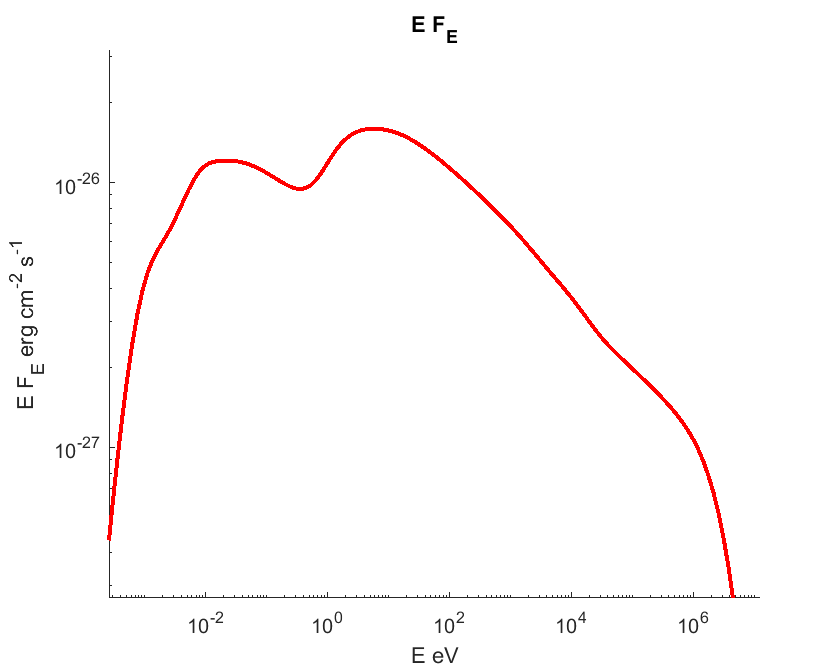
\includegraphics[width=12.5 cm]{./fig/compton.png} 
	\caption{Энергетическая плотность потока синхротронного излучения от тестового источника}
	\label{compton}
\end{figure}

\section{Распад пионов}

Для расчета излучения, получающегося в результате распада пионов, родившихся в результате свободно-свободного взаимодействия протонов использеутся абастрактный класс PionDecayEvaluatorBase и двае его наследника: PionDecayEvaluatorKelner, в котором сечение излучения гамма-фотона считается долей от полного сечения неупругого взаимодействия протонов, как описано в статье \cite{Kelner}, и PionDecayEvaluator, в котором используется более точное описание сечения рождения пионов на низких энергиях по методу, описанному в \cite{Kafexhiu}. В текущей версии предполагается, что характерное время потерь энергии протонов при неупругом взаимодействии намного больше времени их удержания в источнике, система является прозрачной для протонов, и каждый из них взаимодействует не более одного раза. В противном случае используемая модель излучения не применима.

При создании объекта класса PionDecayEvaluator необходимо указать рассматриваемый диапазон энергий частиц и количество точек в нем, а так же концентрацию фоновых протонов, так как предполагается рассеяние высокоэнергичных фотонов на покоящихся, а не взаимодействие высокоэнергичных между собой. Публичные методы класса PionDecayEvaluatorBase и его наследников приведены в Таблице \ref{pionDecay}

		\begin{small}
			\topcaption{Публичные методы классa PionDecayEvaluatorBase и его наследников }
			\label{pionDecay}
			\begin{xtabular}{|p{0.5\textwidth}|p{0.5\textwidth}|}  
				\hline
				\textbf{PionDecayEvaluatorBase} & абстрактный класс для вычисления гамма излучения от распада пионов\\
				\hline
				sigmaInelastic(const double\& energy) & возвращает полное сечение неупругого взаимодействия протонов в лабораторной системе, принимает кинетическую энергию движущегося протона\\
				\hline
				\textbf{PionDecayEvaluatorKelner} & класс для вычисления гамма излучения от распада пионов по методу из статьи \cite{Kelner}\\
				\hline
				PionDecayEvaluatorKelner(int Ne, double Emin, double Emax, const double\& ambientConcentration) & конструктор, создает экземпляр с заданным рассматриваемым диапазоном энергии и концентрацией фоновых протонов\\
				\hline
				\textbf{PionDecayEvaluator} & класс для вычисления гамма излучения от распада пионов по методу из статьи \cite{Kafexhiu}\\
				\hline
				PionDecayEvaluator(int Ne, double Emin, double Emax, const double\& ambientConcentration) & конструктор, создает экземпляр с заданным рассматриваемым диапазоном энергии и концентрацией фоновых протонов\\
				\hline
				sigmaGamma(const double\& photonEnergy, const double\& protonEnergy) & возвращает дифференциальное сечение рождения фотона с данной энергией при данной кинетической энергии протона, усредненное по углам\\
				\hline
			\end{xtabular}
		\end{small}

Пример вычисления излучения от гамма излучения от распада пионов показан в функции evaluatePionDecay() в файлк examples.cpp. В нем рассмотрено моделирование излучение объекта Кокон Лебедя в модели ускорения частиц на вторичных ударных волнах, следуя статье \cite{BykovKalyashova2022}. В данной работе вычислено, что спектр ускоренных протонов имеет вид степенной функции с изломом со следующими параметрами - показатели спектра 2.1 и 2.64 на низких и высоких энергиях соответственно, энергия излома - 2.2 ТэВ. Размер излучающей области брался равным размеру сверхкаверны Лебедя - 55 пк. Как и ранее, сначала определим переменные, задающие основные параметры источника - концентрацию частиц, его размер и магнитное поле, которое опять положим равным нулю. Диапазон энергий протонов рассмотрим от 0.01 ГэВ до 10 ТэВ. Так же укажем энергию излома.
\begin{lstlisting}[language=c++]
	double protonConcentration = 150;
	double rmax = 55 * parsec;
	double B = 0;
	double sinTheta = 1.0;

	double distance = 1400 * parsec;
	double Emin = massProton*speed_of_light2 + 0.01E9 * 1.6E-12;
	double Emax = 1E13 * 1.6E-12;
	double Etrans = 2.2E12 * 1.6E-12;
\end{lstlisting}
После этого создадим распределение протонов и источник излучения
\begin{lstlisting}[language=c++]
	MassiveParticleBrokenPowerLawDistribution* protons = new 
		MassiveParticleBrokenPowerLawDistribution(
		massProton, 2.1, 2.64, Emin, Etrans, protonConcentration);
	RadiationSource* source = new SimpleFlatSource(
		protons, B, sinTheta, rmax, rmax, distance);
\end{lstlisting}
Далее потребуется вычислитель излучения. В случае пионного распада необходимо указать концентрацию фоновых протонов.
\begin{lstlisting}[language=c++]
double protonAmbientConcentration = 20;
PionDecayEvaluator* pionDecayEvaluator = new PionDecayEvaluator(
	200, Emin, Emax, protonAmbientConcentration);
\end{lstlisting}
Как и в предыдущих случаях далее необходимо внутри цикла вычислить излучение в интересующем диапазоне энергий, используя функцию evaluateFluxFromSource, и вывести результат в файл в удобных единицах. Спектр излучения, полученный в результате работы данной программы и результаты наблюдений Кокона Лебедя на Fermi LAT, ARGO и HAWC \cite{Ackermann2011, Bartoli2014, Abeysekara2021} приведены на рисунке \ref{pion}
\begin{figure}
	\centering
	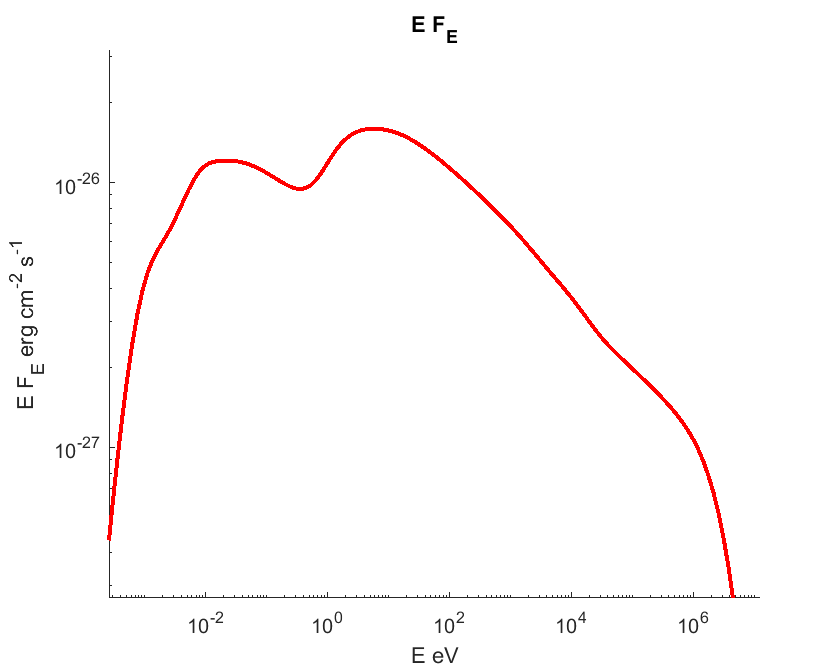
\includegraphics[width=12.5 cm]{./fig/compton.png} 
	\caption{Расчетная энергетическая плотность потока гамма излучения Кокона Лебедя и данные наблюдений}
	\label{pion}
\end{figure}
\section{Тормозное излучение}
В текущей версии кода реализовано вычисление тормозного излучения электронов в плазме только для случая теплового распределения. Для этого предназначен класс BremsstrahlungThermalEvaluator. В процессе расчета предполагается, что плазма электрон-протонная, с одинаковыми температурами электронов и протонов, в вычислении используются Гаунт-факторы, приведенные в \cite{Rybicki}. Пример вычисления тормохного излучения приведен в функции evaluateBremsstrahlung в файле examples.cpp.

